%----------------cost vs. bucketsize--------------------
\begin{figure*}
  \centering
  \subfloat[\covtype]{
  \centering 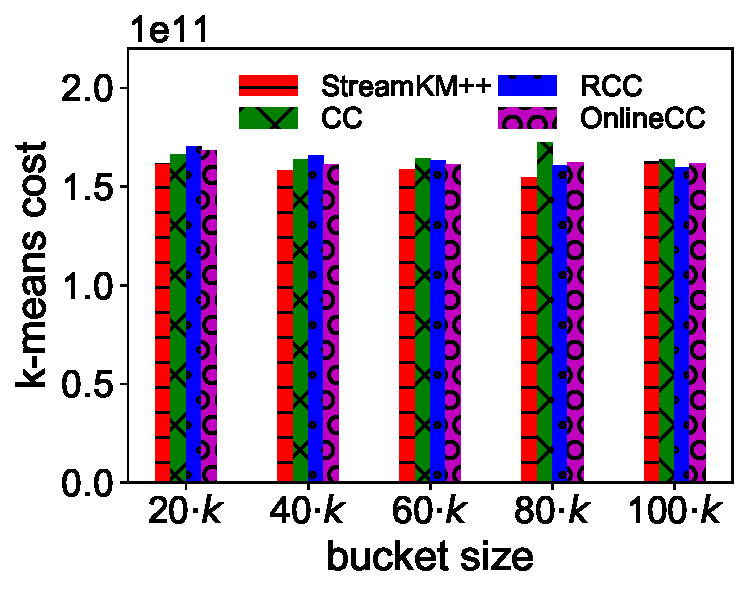
\includegraphics[width=0.23\textwidth]{expfigs/accuracy_bucketsize/covtype_cost_vs_m.pdf}
  }
  \subfloat[\power]{
  \centering 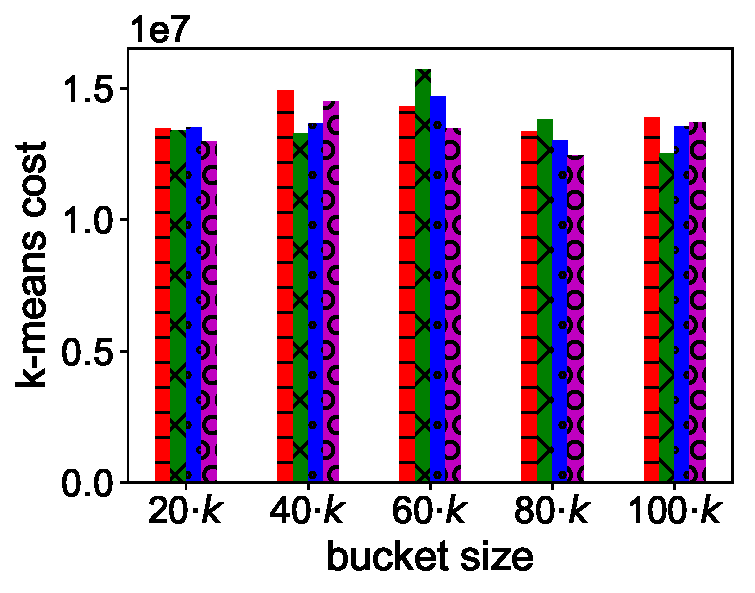
\includegraphics[width=0.23\textwidth]{expfigs/accuracy_bucketsize/power_cost_vs_m.pdf}
  }
  \subfloat[\intrusion]{
  \centering 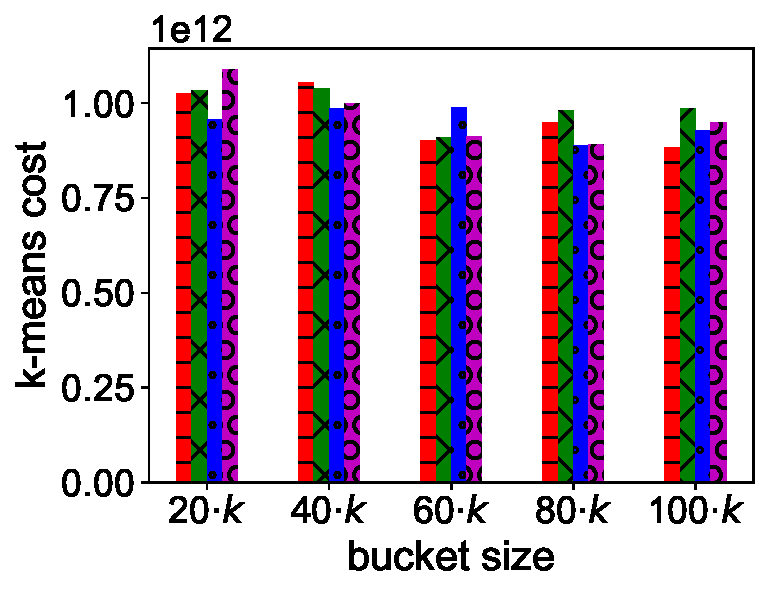
\includegraphics[width=0.23\textwidth]{expfigs/accuracy_bucketsize/intrusion_cost_vs_m.pdf}
  }
  \subfloat[\drift]{
  \centering 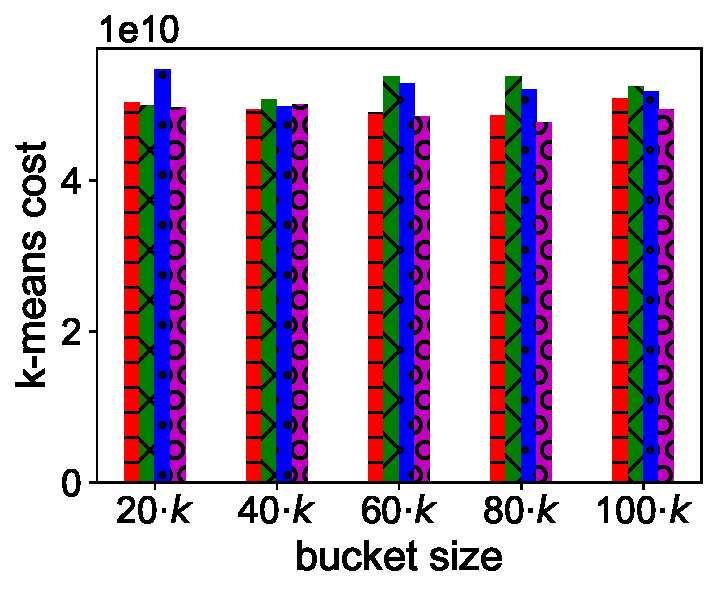
\includegraphics[width=0.23\textwidth]{expfigs/accuracy_bucketsize/synthetic_cost_vs_m.pdf}
  }
  \caption{\km cost vs. bucket size $m$. The cost is computed at the end of observing all the points. The number of clusters $k=30$, query interval $q=100$.  }
 \label{fig:cost-versus-m}
\end{figure*}
%----------------

%----------------update vs. bucketsize--------------------
\begin{figure*}
  \centering
  \subfloat[\covtype]{
  \centering 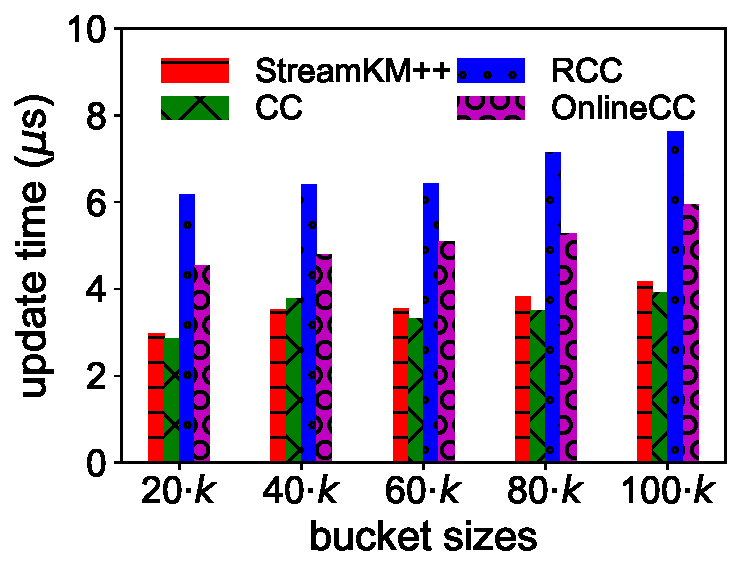
\includegraphics[width=0.23\textwidth]{expfigs/update_bucketsize/covtype_update_vs_m.pdf}
  }
  \subfloat[\power]{
  \centering 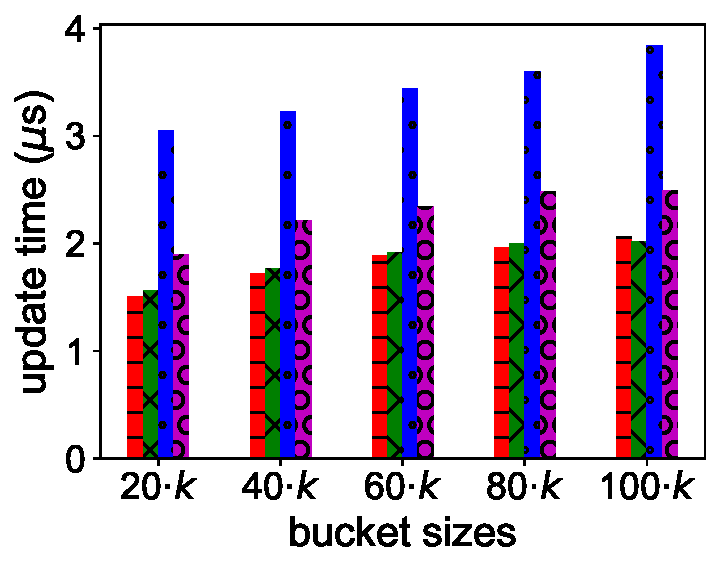
\includegraphics[width=0.23\textwidth]{expfigs/update_bucketsize/power_update_vs_m.pdf}
  }
  \subfloat[\intrusion]{
  \centering 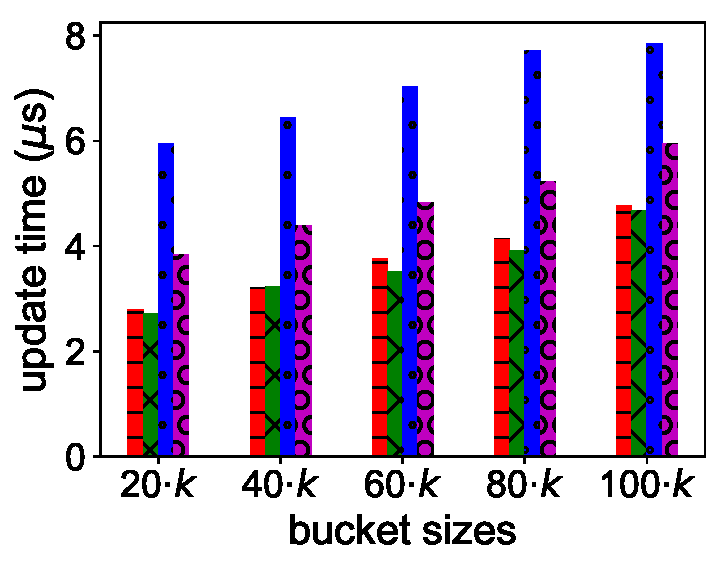
\includegraphics[width=0.23\textwidth]{expfigs/update_bucketsize/intrusion_update_vs_m.pdf}
  }
  \subfloat[\drift]{
  \centering 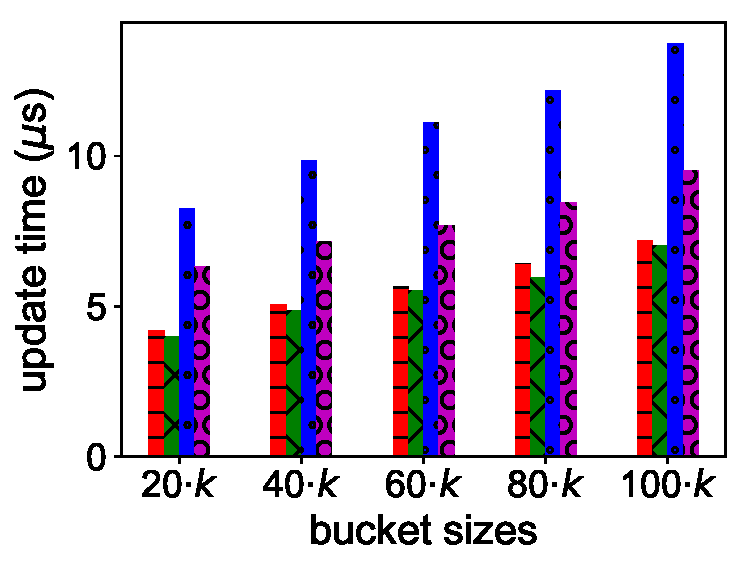
\includegraphics[width=0.23\textwidth]{expfigs/update_bucketsize/synthetic_update_vs_m.pdf}
  }
  \caption{Average update time per point (microseconds)  vs. bucket size $m$. The number of clusters $k=30$, query interval $q=100$.  }
 \label{fig:update-versus-m}
\end{figure*}
%----------------


%----------------query vs. bucketsize--------------------
\begin{figure*}
  \centering
  \subfloat[\covtype]{
  \centering 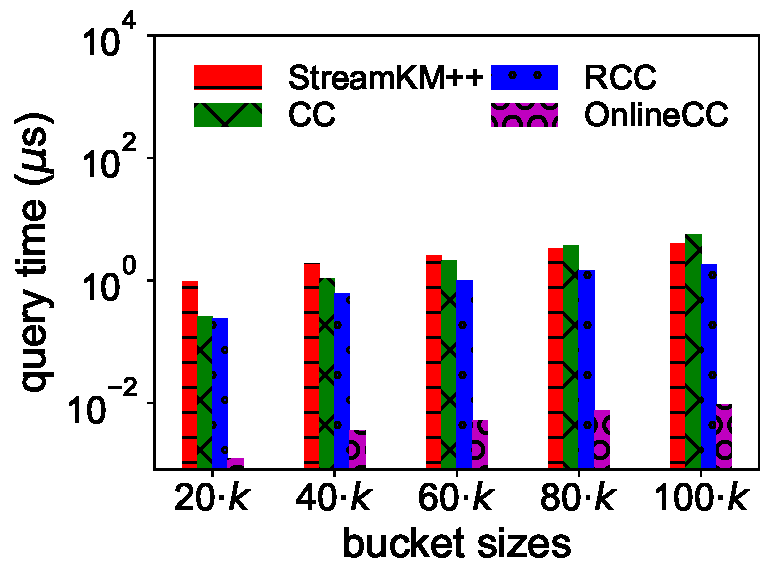
\includegraphics[width=0.23\textwidth]{expfigs/query_bucketsize/covtype_query_vs_m.pdf}
  }
  \subfloat[\power]{
  \centering 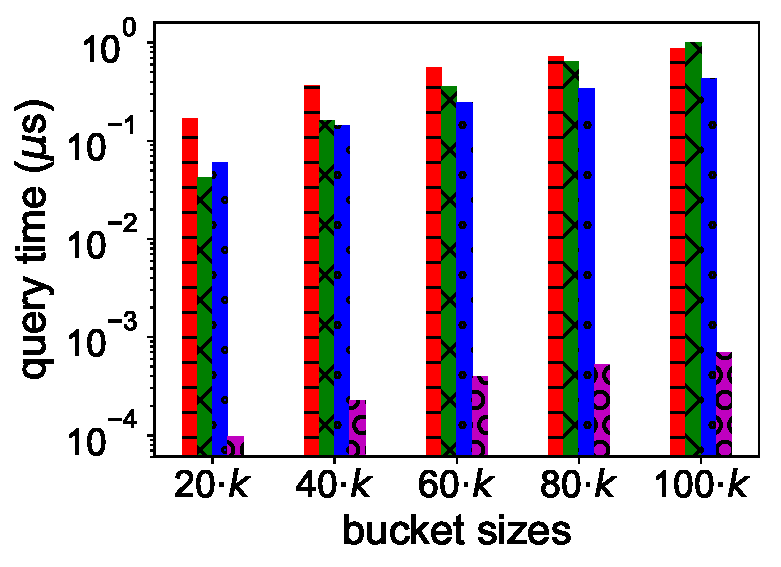
\includegraphics[width=0.23\textwidth]{expfigs/query_bucketsize/power_query_vs_m.pdf}
  }
  \subfloat[\intrusion]{
  \centering 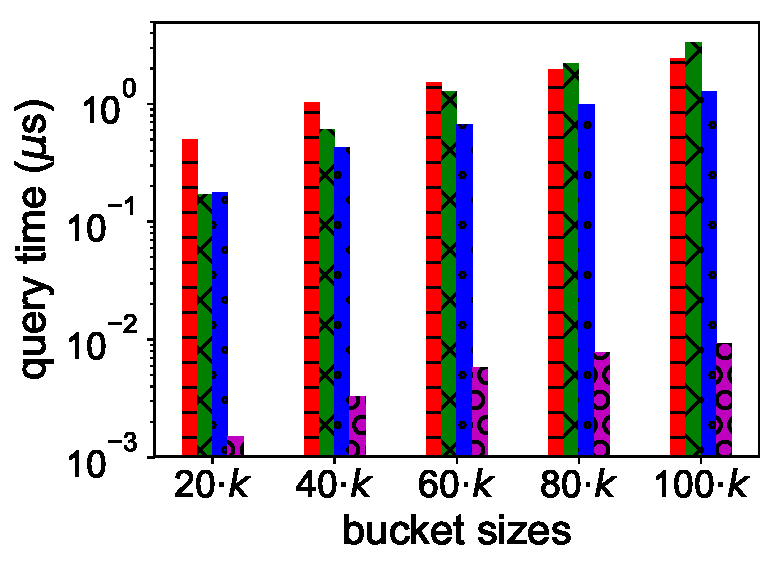
\includegraphics[width=0.23\textwidth]{expfigs/query_bucketsize/intrusion_query_vs_m.pdf}
  }
  \subfloat[\drift]{
  \centering 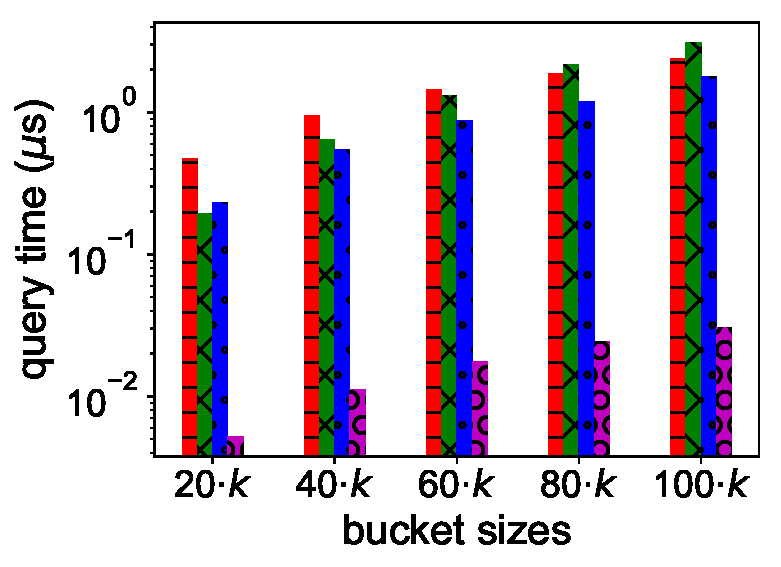
\includegraphics[width=0.23\textwidth]{expfigs/query_bucketsize/synthetic_query_vs_m.pdf}
  }
  \caption{Average query time per point (microseconds) vs. bucket size $m$. The number of clusters $k=30$, query interval $q=100$.  }
 \label{fig:query-versus-m}
\end{figure*}
%-------------------------

%----------------total vs. bucketsize--------------------
\begin{figure*}
  \centering
  \subfloat[\covtype]{
  \centering 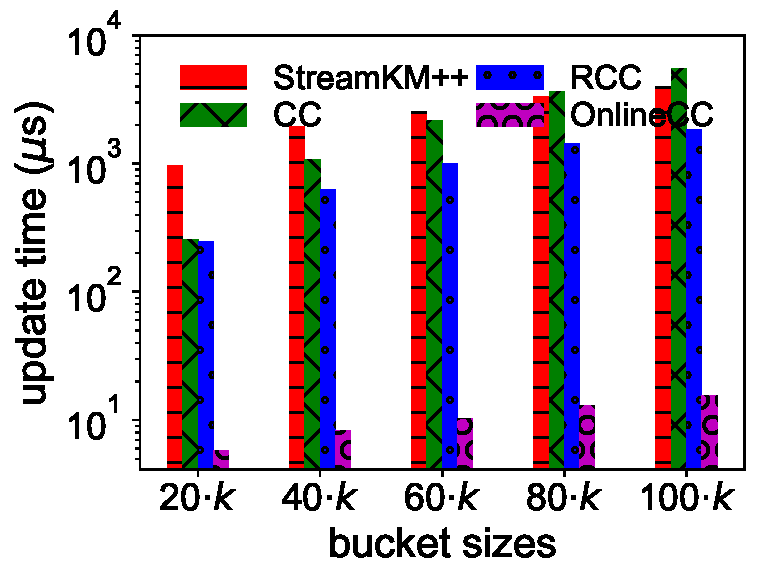
\includegraphics[width=0.23\textwidth]{expfigs/total_bucketsize/covtype_total_vs_m.pdf}
  }
  \subfloat[\power]{
  \centering 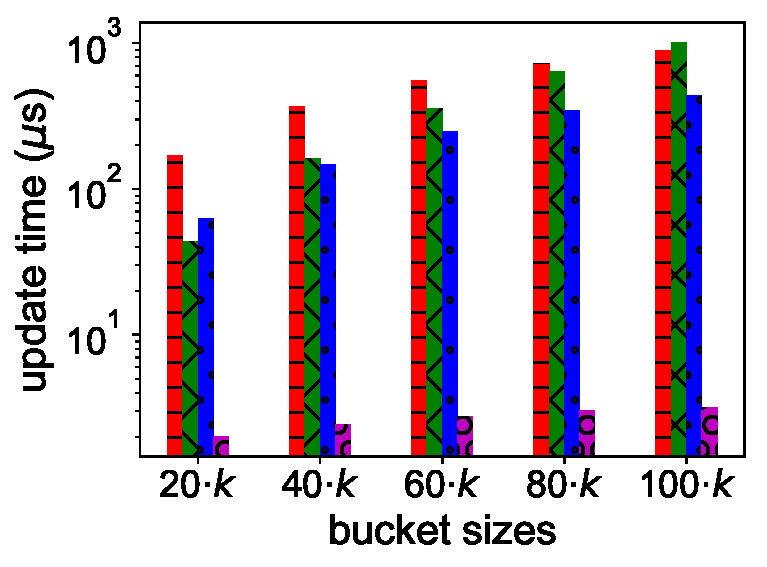
\includegraphics[width=0.23\textwidth]{expfigs/total_bucketsize/power_total_vs_m.pdf}
  }
  \subfloat[\intrusion]{
  \centering 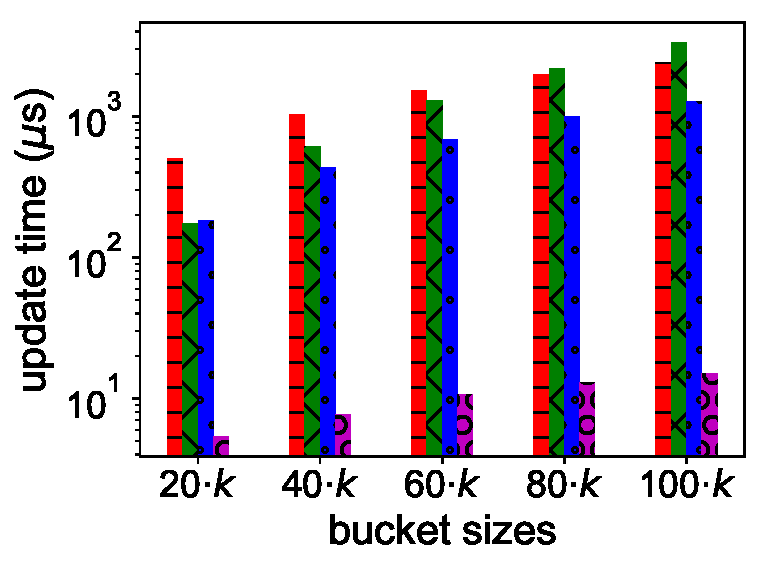
\includegraphics[width=0.23\textwidth]{expfigs/total_bucketsize/intrusion_total_vs_m.pdf}
  }
  \subfloat[\drift]{
  \centering 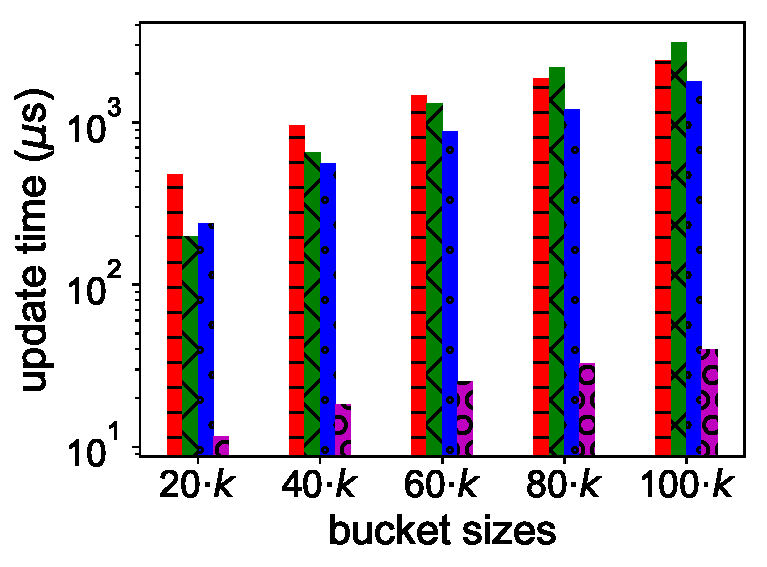
\includegraphics[width=0.23\textwidth]{expfigs/total_bucketsize/synthetic_total_vs_m.pdf}
  }
  \caption{Average runtime per point (microseconds) vs. bucket size $m$. The runtime is the sum of update time (per point) and the query time (per point). The number of clusters $k=30$, query interval $q=100$.  }
 \label{fig:total-versus-m}
\end{figure*}
%-------------------------
